% Chapter 10: Practical Implementation Guide

\section{Practical Implementation}

% Section Introduction
\sectionintro{Practical Implementation}{\faCogs}{From Theory to Production}

% Choosing the Right Embeddings
\begin{conceptslide}{Choosing the Right Embedding Model}{2}
\textbf{Decision Framework for Model Selection}

\begin{columns}
\column{0.5\textwidth}
\textbf{Key Considerations:}

\begin{enumerate}
    \item \concept{Task Requirements}
    \begin{itemize}
        \item Semantic similarity
        \item Classification
        \item Retrieval/Search
        \item Cross-lingual
    \end{itemize}
    
    \item \concept{Resource Constraints}
    \begin{itemize}
        \item Memory: 100MB - 10GB
        \item Latency: 1ms - 100ms
        \item Throughput: 10 - 10K QPS
    \end{itemize}
    
    \item \concept{Data Characteristics}
    \begin{itemize}
        \item Domain specificity
        \item Language coverage
        \item Document length
    \end{itemize}
\end{enumerate}

\column{0.5\textwidth}
\textbf{Decision Tree:}
\begin{center}
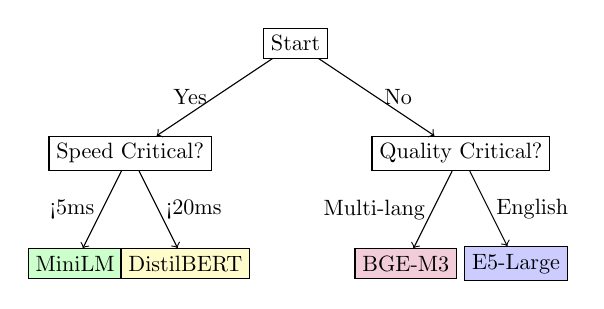
\begin{tikzpicture}[scale=0.7, every node/.style={scale=0.8}]
    % Root
    \node[draw,rectangle] (root) at (0,0) {Start};
    
    % First level
    \node[draw,rectangle] (speed) at (-3,-2) {Speed Critical?};
    \node[draw,rectangle] (quality) at (3,-2) {Quality Critical?};
    
    % Speed branch
    \node[draw,fill=green!20] (fast) at (-4,-4) {MiniLM};
    \node[draw,fill=yellow!20] (medium) at (-2,-4) {DistilBERT};
    
    % Quality branch
    \node[draw,fill=blue!20] (best) at (4,-4) {E5-Large};
    \node[draw,fill=purple!20] (multi) at (2,-4) {BGE-M3};
    
    % Connections
    \draw[->] (root) -- (speed) node[midway,left] {Yes};
    \draw[->] (root) -- (quality) node[midway,right] {No};
    \draw[->] (speed) -- (fast) node[midway,left] {<5ms};
    \draw[->] (speed) -- (medium) node[midway,right] {<20ms};
    \draw[->] (quality) -- (best) node[midway,right] {English};
    \draw[->] (quality) -- (multi) node[midway,left] {Multi-lang};
\end{tikzpicture}
\end{center}

\begin{insightbox}
Start with sentence-transformers library - it has 100+ pre-trained models!
\end{insightbox}
\end{columns}
\end{conceptslide}

% Implementation Pipeline
\begin{conceptslide}{Production Pipeline Architecture}{3}
\textbf{End-to-End Embedding System}

\begin{center}
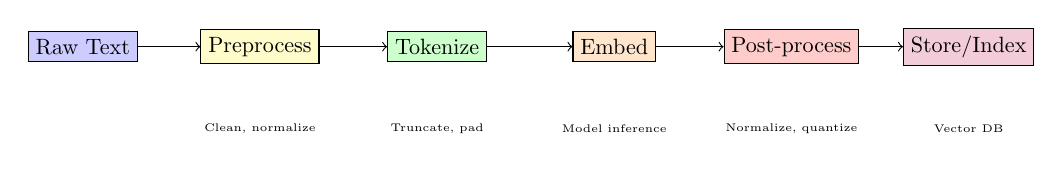
\begin{tikzpicture}[scale=0.9, every node/.style={scale=0.8}]
    % Boxes
    \node[draw,rectangle,fill=blue!20] (input) at (0,0) {Raw Text};
    \node[draw,rectangle,fill=yellow!20] (preprocess) at (2.5,0) {Preprocess};
    \node[draw,rectangle,fill=green!20] (tokenize) at (5,0) {Tokenize};
    \node[draw,rectangle,fill=orange!20] (embed) at (7.5,0) {Embed};
    \node[draw,rectangle,fill=red!20] (postprocess) at (10,0) {Post-process};
    \node[draw,rectangle,fill=purple!20] (store) at (12.5,0) {Store/Index};
    
    % Connections
    \draw[->] (input) -- (preprocess);
    \draw[->] (preprocess) -- (tokenize);
    \draw[->] (tokenize) -- (embed);
    \draw[->] (embed) -- (postprocess);
    \draw[->] (postprocess) -- (store);
    
    % Details below
    \node[below of=preprocess,yshift=-0.3cm] {\tiny Clean, normalize};
    \node[below of=tokenize,yshift=-0.3cm] {\tiny Truncate, pad};
    \node[below of=embed,yshift=-0.3cm] {\tiny Model inference};
    \node[below of=postprocess,yshift=-0.3cm] {\tiny Normalize, quantize};
    \node[below of=store,yshift=-0.3cm] {\tiny Vector DB};
\end{tikzpicture}
\end{center}

\textbf{Key Implementation Steps:}
\begin{columns}
\column{0.33\textwidth}
\textbf{1. Preprocessing:}
\begin{itemize}
    \item Remove HTML/special chars
    \item Handle unicode
    \item Case normalization
    \item Length limits
\end{itemize}

\column{0.33\textwidth}
\textbf{2. Batching Strategy:}
\begin{itemize}
    \item Dynamic batching
    \item Padding optimization
    \item GPU memory management
    \item Async processing
\end{itemize}

\column{0.34\textwidth}
\textbf{3. Storage:}
\begin{itemize}
    \item Vector databases (Pinecone, Weaviate)
    \item FAISS for local
    \item Compression options
    \item Metadata handling
\end{itemize}
\end{columns}
\end{conceptslide}

% Optimization Techniques
\begin{conceptslide}{Optimization Techniques}{4}
\textbf{Making It Fast and Efficient}

\begin{columns}
\column{0.5\textwidth}
\textbf{Speed Optimizations:}

\begin{enumerate}
    \item \concept{Model Optimizations}
    \begin{itemize}
        \item ONNX conversion: 2-3x speedup
        \item TensorRT: 5x on NVIDIA
        \item Quantization: INT8 for 4x speed
    \end{itemize}
    
    \item \concept{Batch Processing}
    \begin{itemize}
        \item Optimal batch size: 32-64
        \item Dynamic padding
        \item Sequence bucketing
    \end{itemize}
    
    \item \concept{Caching Strategies}
    \begin{itemize}
        \item LRU cache for common queries
        \item Precompute frequent documents
        \item Warm start on deployment
    \end{itemize}
\end{enumerate}

\column{0.5\textwidth}
\textbf{Memory Optimizations:}

\begin{mathbox}
\textbf{Memory Formula:}
$$M = V \times D \times P \times B$$
where:
\begin{itemize}
    \item $V$ = Vocabulary size
    \item $D$ = Embedding dimension
    \item $P$ = Precision (4 bytes for FP32)
    \item $B$ = Batch size
\end{itemize}
\end{mathbox}

\textbf{Reduction Techniques:}
\begin{center}
\begin{tabular}{lcc}
\toprule
Technique & Memory & Speed \\
\midrule
FP32 → FP16 & 50\% & 1.5x \\
Quantization & 25\% & 2x \\
Pruning & 40\% & 1.2x \\
Distillation & 10\% & 3x \\
\bottomrule
\end{tabular}
\end{center}

\begin{trybox}
Combine techniques: FP16 + ONNX + batching = 10x speedup!
\end{trybox}
\end{columns}
\end{conceptslide}

% Fine-tuning Strategies
\begin{conceptslide}{Fine-tuning for Your Domain}{3}
\textbf{Adapting Pre-trained Models}

\begin{columns}
\column{0.5\textwidth}
\textbf{When to Fine-tune:}
\begin{itemize}
    \item Domain-specific vocabulary
    \item Unique similarity requirements
    \item Performance below 80\% baseline
    \item Sufficient training data (>10K examples)
\end{itemize}

\vspace{0.3cm}
\textbf{Fine-tuning Approaches:}
\begin{enumerate}
    \item \concept{Full Fine-tuning}
    \begin{itemize}
        \item Update all parameters
        \item Best performance
        \item Risk of overfitting
    \end{itemize}
    
    \item \concept{Adapter Layers}
    \begin{itemize}
        \item Add small trainable layers
        \item Preserve base knowledge
        \item Memory efficient
    \end{itemize}
    
    \item \concept{Contrastive Fine-tuning}
    \begin{itemize}
        \item Use domain pairs
        \item SimCSE approach
        \item No labels needed
    \end{itemize}
\end{enumerate}

\column{0.5\textwidth}
\textbf{Fine-tuning Recipe:}

\begin{algorithm}[H]
\SetAlgoLined
\KwIn{Pre-trained model $M$, Domain data $D$}
\KwOut{Fine-tuned model $M'$}
\BlankLine
1. Prepare pairs from $D$\;
2. Initialize $M'$ ← $M$\;
3. Freeze bottom layers\;
\For{epoch in 1..N}{
    \For{batch in $D$}{
        Compute embeddings\;
        Calculate contrastive loss\;
        Update top layers only\;
    }
    Evaluate on validation\;
    \If{improved}{
        Save checkpoint\;
    }
}
\Return{Best checkpoint}
\end{algorithm}

\begin{warningbox}
Always validate on held-out data - overfitting is common!
\end{warningbox}
\end{columns}
\end{conceptslide}

% Deployment Patterns
\begin{conceptslide}{Deployment Patterns}{3}
\textbf{From Development to Production}

\begin{columns}
\column{0.5\textwidth}
\textbf{Architecture Patterns:}

\begin{enumerate}
    \item \concept{Microservice Pattern}
    \begin{itemize}
        \item Embedding service API
        \item Horizontal scaling
        \item Language agnostic
    \end{itemize}
    
    \item \concept{Sidecar Pattern}
    \begin{itemize}
        \item Co-located with app
        \item Low latency
        \item Resource sharing
    \end{itemize}
    
    \item \concept{Edge Deployment}
    \begin{itemize}
        \item Model on device
        \item Privacy preserving
        \item Offline capability
    \end{itemize}
\end{enumerate}

\column{0.5\textwidth}
\textbf{Production Checklist:}

\begin{itemize}
    \item[\faCheckSquare] Model versioning system
    \item[\faCheckSquare] A/B testing framework
    \item[\faCheckSquare] Monitoring \& alerting
    \item[\faCheckSquare] Fallback mechanisms
    \item[\faCheckSquare] Load balancing
    \item[\faCheckSquare] Cache warming
    \item[\faCheckSquare] Rate limiting
    \item[\faCheckSquare] Security (API keys, encryption)
\end{itemize}

\textbf{Monitoring Metrics:}
\begin{itemize}
    \item Latency P50, P95, P99
    \item Throughput (QPS)
    \item Error rates
    \item Cache hit ratio
    \item Model drift detection
\end{itemize}
\end{columns}

\vspace{0.5cm}
\begin{center}
\colorbox{alertSuccess!20}{\parbox{0.9\textwidth}{
\textbf{Pro Tip:} Start with a simple REST API, then optimize based on actual usage patterns!
}}
\end{center}
\end{conceptslide}

% Common Pitfalls
\begin{frame}{Common Pitfalls and Solutions}
\textbf{Learn from Others' Mistakes}

\begin{columns}
\column{0.5\textwidth}
\textbf{\faWarning\ Common Mistakes:}

\begin{enumerate}
    \item \concept{Wrong Similarity Metric}
    \begin{itemize}
        \item Using L2 instead of cosine
        \item Not normalizing embeddings
        \item Solution: Always test both!
    \end{itemize}
    
    \item \concept{Tokenization Mismatch}
    \begin{itemize}
        \item Different tokenizers in train/inference
        \item Truncation issues
        \item Solution: Save tokenizer with model
    \end{itemize}
    
    \item \concept{Version Drift}
    \begin{itemize}
        \item Model updates break compatibility
        \item Embedding dimension changes
        \item Solution: Versioned embeddings
    \end{itemize}
\end{enumerate}

\column{0.5\textwidth}
\textbf{\faLightbulbO\ Best Practices:}

\begin{enumerate}
    \item \textbf{Always Benchmark}
    \begin{itemize}
        \item Test on your actual data
        \item Measure end-to-end latency
        \item Track quality metrics
    \end{itemize}
    
    \item \textbf{Progressive Rollout}
    \begin{itemize}
        \item Start with 1\% traffic
        \item Monitor closely
        \item Gradual increase
    \end{itemize}
    
    \item \textbf{Maintain Backwards Compatibility}
    \begin{itemize}
        \item Support multiple versions
        \item Graceful degradation
        \item Migration tools
    \end{itemize}
\end{enumerate}

\begin{insightbox}
The best embedding model is the one that works for YOUR specific use case!
\end{insightbox}
\end{columns}
\end{frame}